% Copyright (c)  2010-2011  EDF-EADS.
% Permission is granted to copy, distribute and/or modify this document
% under the terms of the GNU Free Documentation License, Version 1.2
% or any later version published by the Free Software Foundation;
% with no Invariant Sections, no Front-Cover Texts, and no Back-Cover
% Texts.  A copy of the license is included in the section entitled "GNU
% Free Documentation License".

\documentclass[11pt]{article}

\usepackage{OTAgrumDocumentation}
\usepackage{Math_Notations}

\makeindex

\begin{document}

\thispagestyle{empty}

% Copyright (c)  20010  EDF-EADS.
% Permission is granted to copy, distribute and/or modify this document
% under the terms of the GNU Free Documentation License, Version 1.2
% or any later version published by the Free Software Foundation;
% with no Invariant Sections, no Front-Cover Texts, and no Back-Cover
% Texts.  A copy of the license is included in the section entitled "GNU
% Free Documentation License".
\vspace*{2cm}

\begin{center}
  {\huge \bf Documentation of the OpenTURNS-aGrUM module}
  \input{GenericInformation.tex}
\end{center}



\newpage
%  Copyright (c)  2005-2009  EDF-EADS.
%  Permission is granted to copy, distribute and/or modify this document
%  under the terms of the GNU Free Documentation License, Version 1.2
%  or any later version published by the Free Software Foundation;
%  with no Invariant Sections, no Front-Cover Texts, and no Back-Cover
%  Texts.  A copy of the license is included in the section entitled "GNU
%  Free Documentation License".
\vspace{0.5in}
\begin{center}
\vspace{0.3in}
\emph{\fontshape{sc} Abstract}
\vspace{0.5in}
\end{center}

The purpose of this document is to present the OpenTURNS-aGrUM module, which enables to define Bayesian networks with aGrUM and to manipulate them with OpenTURNS.

It offers to the user the ability to:
\begin{itemize}
\item define discretized aGrUM distributions from OpenTURNS distributions
\item build OpenTURNS objects from aGrUM Bayesian networks
\item extract marginal distributions of aGrUM Bayesian networks as OpenTURNS distributions
\end{itemize}
This document is organised according to the Open TURNS documentation : 
\begin{itemize}
\item a \itshape{Reference Guide} which gives some theoretical basis on bayseian networks,
\item a \itshape{Use cases Guide} which details scripts in python (the Textual Interface langage of Open TURNS) and helps the User to learn as quickly as possible the manipulation of the $otagrum$ module,
\item the \itshape{User Manual} which details the $otagrum$ objects and give the list of their methods,
\item the \itshape{Examples Guide} which provides at the moment only one example performed with the  $otagrum$ module.
\end{itemize}

\tableofcontents
\newpage
% Copyright (c)  2010-2011  EDF-EADS.
% Permission is granted to copy, distribute and/or modify this document
% under the terms of the GNU Free Documentation License, Version 1.2
% or any later version published by the Free Software Foundation;
% with no Invariant Sections, no Front-Cover Texts, and no Back-Cover
% Texts.  A copy of the license is included in the section entitled "GNU
% Free Documentation License".




%%%%%%%%%%%%%%%%%%%%%%%%%%%%%%%%%%%%%%%%%%%%%%%%%%%%%%%%%%%%%%%%%%%%%%%%%%%%%%%%%%%%%%%%%% 
\section{Reference Guide}

The aGrUM library provides efficient algorithms to create and manipulate graphical models. A particular case of such models is the class of Bayesian Networks (BN), which is of first interest in association with OpenTURNS.

\subsection{Bayesian networks}

The following lines are partially extracted from the Wikipedia Encyclopedia. For an in-deepth presentation of the BN theory and algorithms, the reader could read the references indicated in   section \ref{ref}.\\

A {\itshape Bayesian network}, {\itshape belief network} or {\itshape directed acyclic graphical model} is a probabilistic graphical model that represents a set of random variables and their conditional dependencies via a directed acyclic graph (DAG). In this DAG, edges represent conditional dependencies; nodes which are not connected represent variables which are conditionally independent of each other. Each node is associated with a probability function that takes as input a particular set of values for the node's parent variables and gives the probability of the variable represented by the node. \\

The manipulation of a Baysesian network is called {\itshape inference}. Efficient algorithms exist that perform inference and learning in Bayesian networks. 


\subsection{References and theoretical basis}\label{ref}

\begin{itemize}
  \item[1] {\itshape Reseaux Bay�siens - aGrUM}, PH. Wuillemin, Journ�e Utilisateurs Open TURNS 2010, http://share.openturns.org
  \item[2] to precise 
  \item[3]  Wikipedia, www.wikipedia.org, reserach word 'Bayesian Network'
\end{itemize}
\newpage
% Copyright (c)  2010-2011  EDF-EADS.
% Permission is granted to copy, distribute and/or modify this document
% under the terms of the GNU Free Documentation License, Version 1.2
% or any later version published by the Free Software Foundation;
% with no Invariant Sections, no Front-Cover Texts, and no Back-Cover
% Texts.  A copy of the license is included in the section entitled "GNU
% Free Documentation License".




%%%%%%%%%%%%%%%%%%%%%%%%%%%%%%%%%%%%%%%%%%%%%%%%%%%%%%%%%%%%%%%%%%%%%%%%%%%%%%%%%%%%%%%%%% 
\section{Use Cases Guide}

This section presents the main functionalities of the module $otagrum$ in their context. As the module  $otagrum$ links the $openturns$ objects and the $pyagrum$ ones, we precise for each script from which library the python lines come from.\\
It is possible to have more exhaustive information on the $pyagrum$ module on the web site $http://agrum.lip6.fr$.



%%%%%%%%%%%%%%%%%%%%%%%%%%%%%%%%%%%%%%%%%%%%%%%%%%%%%%%%%%%%%%
\subsection{Which python modules to import ?}

In order to use the functionalities described in this documentation, it is necessary to import  : 
\begin{itemize}
   \item the $openturns$ python module which gives access to the Open TURNS functionalities,
   \item the $pyAgrum$ module which gives access to the aGrUM functionalities,
   \item the $otagrum$ module which links the $openturns$ functionalities and the $pyAgrum$ ones.
\end{itemize}

Python  script for this use case :

\begin{lstlisting}
# Load OpenTURNS to manipulate distributions
from openturns import *
# Load pyAgrum to define the Network
from pyAgrum import *
# Load the link between OT and aGrUM
from otagrum import *
\end{lstlisting}

%%%%%%%%%%%%%%%%%%%%%%%%%%%%%%%%%%%%%%%%%%%%%%%%%%%
\newpage \subsection{Creation of a Variable} \label{VariableCreation}

In $pyagrum$, it is possible to create three different kinds of discrete variables : 
\begin{itemize} 
  \item a categorial variable which labels are strings : the $LabelizedVar$,
  \item a discrete variable which range is a finite interval of $\mathbb{N}$ : the $RangeVar$,
  \item a discretized variable which is a real variable which range is discretized into a finite collection of intervals of $\mathbb{R}$ : $([T_0, T_1], \hdots, [T_{N-1}, T_N])$, where $T_O$ can be equal to $-\infty$ and
    $T_N$ equal to $+\infty$ : the $DiscretizedVar$.
\end{itemize}

%%%%%%%%%%%%%%%%%%%%%%%%%%%%%%%%%%%%%%%%%%%%%%%%%%%%%%%%%%%%%%
\subsubsection{UC : Creation of a Categorical Variable}

A categorical variable is a discrete variable which modalities are considered as labels. It may be some strings or even some numbers but considered as special strings.\\

This use case shows how to create such a variable : creation of the object and its modalities. The quantification step is described further in section \ref{BayesNetQuantification}.\\

The following lines are entirely part of the $pyagrum$ module. \\

\requirements{
  \begin{description}
  \item[$\bullet$] none
  \end{description}
}
{
  \begin{description}
  \item[$\bullet$] a Categorical variable  : {\itshape myCategoricalVar},
  \item[type:] a LabelizedVar
  \end{description}
}

\espace
Python  script for this use case :

\begin{lstlisting}
# Create a categorical variable

# Choose a name
name = 'light'
# Give a comment
comment = 'Intensity of the light'
# Fix the initial number of modalities to 0
initialNumberModalities = 0
myCategoricalVar = LabelizedVar(name, comment, initialNumberModalities)

# Add your labels : for example 3 labels
myCategoricalVar.addLabel("modality1")
myCategoricalVar.addLabel("modality2")
myCategoricalVar.addLabel("modality3")

# Print the created categorical variable
print myCategoricalVar

# Explicitate the label number i
# Care : numerotation begins at 0
print myCategoricalVar.label(2)

# Explicitate all the labels
print myCategoricalVar.labels()

# Erase all the declared labels 
# the categorical variable has no label any more
myCategoricalVar.eraseLabels()
\end{lstlisting}



%%%%%%%%%%%%%%%%%%%%%%%%%%%%%%%%%%%%%%%%%%%%%%%%%%%%%%%%%%%%%%
\newpage \subsubsection{UC : Creation of a Discrete Variable }

The considered discrete variables have a finite interval of $\mathbb{N}$ as range. \\

This use case shows how to create such a variable : creation of the object and its modalities. The quantification step is described further in section \ref{BayesNetQuantification}.\\

The following lines are entirely part of the $pyagrum$ module.\\ 

\requirements{
  \begin{description}
  \item[$\bullet$] none
  \end{description}
}
{
  \begin{description}
  \item[$\bullet$] a discrete variable  which range is a finite interval of $\mathbb{N}$ : {\itshape myDiscreteVar},
  \item[type:] a RangeVar
  \end{description}
}

\espace
Python  script for this UseCase :

\begin{lstlisting}
# Create a discrete variable

# Choose a name
name = 'light'
# Give a comment
comment = 'Intensity of the light'
# Fix the lower and upper bounds of the range
# for example, the range is [3,5]
minRange = 3
maxRange = 5
myDiscreteVar = RangeVar(name, comment, minRange, maxRange)

# Print the created discrete variable
print myDiscreteVar

# Calculate the lenght of the range
lenght = len(myDiscreteVar)

# Test whether the integer i is within the range
print myDiscreteVar.belongs(i)

# Explicitate the label number i
# Care : numerotation begins at 0
print myDiscreteVar.label(2)
\end{lstlisting}


%%%%%%%%%%%%%%%%%%%%%%%%%%%%%%%%%%%%%%%%%%%%%%%%%%%%%%%%%%%%%%
\newpage \subsubsection{UC : Creation of a Discretized Variable}

A discretized variable is a real variable which range is discretized into a finite subset of intervals which bounds are : $(T_0,T_1, \hdots, T_N)$ for $N \in \mathbb{N}$. \\

In the particular case where the variable depends on other ones of the bayesian network, its probability table is composed of several probability tables which might have different discretizations. Thus, it is necessary to find out a global discretization of the variable which is adapted to all the conditional situations of the variable. The $otagrum$ module proposes a method that finds out that global discretization from the given conditional probability distributions.\\

For example, in the  situation drawn in Fig.\ref{BNPlant}, the  $Height$ variable is a discretized one which  depends on the categorical variables $Light$ and $Moisture$. If we suppose that $Light$ has two labels : $Dim$ and $Bright$, and that $Moisture$ have the labels : $Wet$ and $Dry$, then the conditional probability table  of $Height$ is defined as in Tab.\ref{condTP2}.\\

\begin{figure}[H]
\begin{center}
    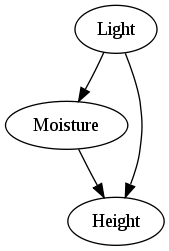
\includegraphics[scale=0.85]{PlantGrowth.png}
    \caption{Bayes Net considered within a plant growth study}
    \label{BNPlant}
  \end{center}
\end{figure}




It is necessary to adapt the Height discretization to the specific conditional distributions $(heightWhenDimAndWet$, $heightWhenBrightAndWet$, $heightWhenDimAndDry$, $heightWhenBrightAndDry$, thanks to the static method $AdaptGrid$ of the object $BayesNetAgrum$ proposed by the $otagrum$ python module.  The adaptation consists in adding, if necessary, some lower and upper bounds to the initial proposed grid so that all the probabilistic mass of  the conditional distributions be included in the final proposed grid. These lower and upper bounds are respectively the min and max of all the numerical lower and upper bounds of the conditional distributions. Furthermore, the initial grid may be potentially unsorted : the final grid is sorted.\\


This use case shows how to create such a variable : creation of the object and its modalities.\\

The corresponding lines are entirely part of the $pyagrum$ module, except for the adaptation of the global discretization which is only supported by the  $otagrum$ module.\\

 The quantification step is described further in section \ref{BayesNetQuantification}.\\

\requirements{
  \begin{description} 
  \item[$\bullet$] some conditional probability distributions : {\itshape dist1, dist2, dist3, dist4}
  \item[type:] Distribution, the $openturns$ object
  \end{description}
}
{
  \begin{description}
  \item[$\bullet$] a discretized variable  : {\itshape myDiscreteVar},
  \item[type:] a DiscretizedVar
  \end{description}
}



\espace

Python  script for this use case :

\begin{lstlisting}
# Create a Discretized variable

# Choose a name
name = 'MyName'
# Give a comment
comment = 'What I represent'
myDiscretizedVar = DiscretizedVar(name, comment)

###########################################################
# CASE 1 : The variable does not depend on other variables
###########################################################

# Give the suite of the interval bounds
# for example, the intervals are [0,1], [1, 3], [3, 10]
myDiscretizedVar.addTick(0)
myDiscretizedVar.addTick(1)
myDiscretizedVar.addTick(3)
myDiscretizedVar.addTick(10)



###################################################################
# CASE 2 : The variable depends on other variables
# Its conditional probability table depends on  4 conditional 
# distributions
# ==> You need to adapt the ticks to the conditional distributions
###################################################################

# Give a first proposition of bounds
# for example, initialData = (0,10,20, ..., 100)
initialTicks = NumericalPoint(range(0, 100, 10))

# Adapt the initial ticks to (dist1, dist2, dist3, dist4)
# Create a collection of distribution
finalTicks = BayesNetAgrum.AdaptGrid(
            DistributionCollection([dist1, dist2, dist3, dist4]), 
            initialTick)

# Set these new adapted ticks to the DiscretizedVar
for i in finalTicks : 
  myDiscretizedVar.addTick(i)

###########################################################

# Print the created discretized variable
print myDiscretizedVar

# Calculate the lenght of the range
lenght = len(myDiscretizedVar)

# Erase all the declared bounds
# the discretized variable has no range any more
myDiscretizedVar.eraseTicks()

# Test whether the real value is one of the range bounds suite
value = 3.4
print myDiscretizedVar.isTick(value)

# Explicitate the intervale [T_i, T_{i+1}]
i=2
print myDiscretizedVar.label(i)
\end{lstlisting}




%%%%%%%%%%%%%%%%%%%%%%%%%%%%%%%%%%%%%%%%%%%%%%%%%%%%%%%%%%%%%%
\newpage \subsection{Creation of a $pyagrum$ Bayes Net} \label{BayesNetCreation}



Once the variables have been created with their modalities as described in section \ref{VariableCreation}, the next step is to create a bayesian network through the $pyagrum$ module line commands, thanks to the object $BayesNet$. \\

It is important to note that the bayesian network object $BayesNet$ can be transformed into the bayesian network object $BayesNetAgrum$ proposed by $otagrum$ only once the $pyagrum$ object has been entirely quantified as described in section \ref{BayesNetQuantification}.\\

%%%%%%%%%%%%%%%%%%%%%%%%%%%%%%%%%%%%%%%%%%%%%%%%%%%%%%%%%%%%%%
\subsubsection{UC : Creation of the graph}

This use case shows how to create the graph of a bayesian network. It takes the example of the structure drawn in Fig.\ref{BNPlant}.\\

The corresponding lines are entirely part of the $pyagrum$ module. \\



\requirements{
  \begin{description} 
  \item[$\bullet$] some variables {\itshape moisture}, {\itshape light}, {\itshape height}
  \item[type:]  a LabelizedVar, a RangeVar or a Discretizedvar
  \end{description}
}
{
  \begin{description}
  \item[$\bullet$] a   $pyagrum$ bayesian network : {\itshape myBNpyagrum},
  \item[type:] a BayesNet
  \end{description}
}

\espace 
Python  script for this use case :

\begin{lstlisting}
# Create an empty bayesian network
netName = "Plant Growth"
myBNpyagrum = BayesNet(netName)

# Add variables to the bayesian network
indexLight    = myBNpyagrum.add(light)
indexMoisture = myBNpyagrum.add(moisture)
indexHeight   = myBNpyagrum.add(height)

# Create arcs
# Light -> Moisture
myBNpyagrum.insertArc(indexLight, indexMoisture)
#  Light -> Height
myBNpyagrum.insertArc(indexLight, indexHeight)
#  Moisture -> Height
myBNpyagrum.insertArc(indexMoisture, indexHeight)

# Print the created Bayes network
print myBNpyagrum

# Show the antecedents of moisture in the order in which they were created
print "moisture Antecedents= ", myBN.cpt(indexMoisture).var_names

# Erase a specific arc
# For example between Light and Moisture
myBNpyagrum.eraseArc(indexLight, indexMoisture)
\end{lstlisting}






%%%%%%%%%%%%%%%%%%%%%%%%%%%%%%%%%%%%%%%%%%%%%%%%%%%%%%%%%%%%%%
\newpage \subsection{Quantification of a Bayes Net} \label{BayesNetQuantification}


The quantification of a bayesian network consists in fulfilling the conditionnal probability table of each variable of the network. There are two different situations : 
\begin{itemize}
   \item the variable has no antecedent, and its probability table does not depend on the realization of other variables,
   \item the variable has at least one antecedent and its probability table is conditonned to the realization of its antecedent(s).
\end{itemize}


%%%%%%%%%%%%%%%%%%%%%%%%%%%%%%%%%%%%%%%%%%%%%%%%%%%%%%%%%%%%%%
\subsubsection{UC : Quantification of a Probability table }

This use case shows how to quantify the probability table of a variable which has no antecedent.\\

The corresponding lines are entirely part of the $pyagrum$ module. \\



\requirements{
  \begin{description} 
  \item[$\bullet$] a   $pyagrum$ bayesian network : {\itshape myBNpyagrum},
  \item[type:] a BayesNet
  \item[$\bullet$] one of its variable {\itshape light} with two modalities, 
  \item[type] a LabelizedVar, a RangeVar or a Discretizedvar
  \end{description}
}
{
  \begin{description}
  \item[$\bullet$] the quantified BayesNet : {\itshape myBNpyagrum},
  \item[type:] a BayesNet
  \end{description}
}

\espace 
Python  script for this use case :

\begin{lstlisting}
# Here we explicitate a line which has been declared previously
# at the creation step of myBNpyagrum
indexLight = myBNpyagrum.add(light)

# Fulfill the probability table
# Modalities are sorted in the order where they were created
# for example, Proba(light== first modality) = 0.25
# for example, Proba(light== second modality) = 0.75
myBNpyagrum.cpt(indexLight)[:]= [0.25, 0.75]
\end{lstlisting}


%%%%%%%%%%%%%%%%%%%%%%%%%%%%%%%%%%%%%%%%%%%%%%%%%%%%%%%%%%%%%%
\newpage \subsubsection{UC : Quantification of a Conditional Probability table }

This use case shows how to quantify the conditional probability table  of a variable which has at least one antecedent.\\

Several cases are treated : 
\begin{itemize}
  \item the variable is a LabelizedVar (or a RangeVar),
  \item the variable is a DiscretizedVar.
\end{itemize}


The corresponding lines are  part of the $pyagrum$ module in the fisrt case.  The second case requires the use of $otagrum$ which proposes the method $BayesNetAgrum.Discretize$ to discretize a continuous distribution of $openturns$ in order to fulfill the conditional probability table of the $pyagrum$ variable.\\

This use case illustrates the example of Fig.\ref{BNPlant}. We suppose the conditionnal probability table described in Tab.\ref{condTP2}.\\

\begin{table}[H]
  \begin{center}
    \begin{tabular}{c|c|c}
      $Moisture$ - $Light$ & $Dim$ & $Bright$ \\
      \hline
      $Wet$ & heightWhenDimAndWet &  heightWhenBrightAndWet\\
      \hline
      $Dry$ & heightWhenDimAndDry &  heightWhenBrightAndDry
    \end{tabular}
    \caption{Example of a conditional table of probability.}
    \label{condTP2}
  \end{center}
\end{table}


\requirements{
  \begin{description} 
  \item[$\bullet$] a   $pyagrum$ bayesian network : {\itshape myBNpyagrum},
  \item[type:] a BayesNet
  \item[$\bullet$] its variables {\itshape light} and {\itshape moisture}  
  \item[type] a LabelizedVar 
  \item[$\bullet$] its variable {\itshape height} 
  \item[type] a DiscretizedVar
  \item[$\bullet$] some  distributions {\itshape heightWhenDimAndWet, ...} 
  \item[type] some $openturns$ Distribution
  \end{description}
}
{
  \begin{description}
  \item[$\bullet$] the quantified BayesNet : {\itshape myBNpyagrum},
  \item[type:] a BayesNet
  \end{description}
}

\espace 
Python  script for this use case :

\begin{lstlisting}
# Here we explicitate some lines which have been declared previously
# at the creation step of myBNpyagrum
indexMoisture = myBNpyagrum.add(moisture)
indexHeight = myBNpyagrum.add(height)

# We show the antecedents of these variables with the order in which they were created
print "Moisture Antecedents= ", myBNpyagrum.cpt(indexMoisture).var_names
print "Height Antecedents= ", myBNpyagrum.cpt(indexHeight).var_names




######################################################################
# CASE 1 : The  LabelizedVar (or RangeVar) depends on a Labelized one
######################################################################
# Fulfill the probability table when light='Dim'
# we recall that the name of light is Light
myBNpyagrum.cpt(indexMoisture)[{'Light' : 'Dim'}] = [0.2, 0.8]

# Fulfill the probability table when light='Bright'
myBNpyagrum.cpt(indexMoisture)[{'Light' : 'Bright'}] = [0.6, 0.4]


######################################################################
# CASE 2 : The  LabelizedVar (or RangeVar)  depends on a RangeVar 
######################################################################
# Fulfill the  probability table when myRangeVar= its first modality (it means 3)
myBNpyagrum.cpt(indexMoisture)[{'nameRange' : 0}]= [0.2, 0.8]

# Fulfill the  probability table when myRangeVar= its second modality (it means 4)
myBNpyagrum.cpt(indexMoisture)[{'nameRange' : 1}]= [0.2, 0.8]

# Fulfill the  probability table when myRangeVar= its third modality (it means 5)
myBNpyagrum.cpt(indexMoisture)[{'nameRange' : 2}]= [0.2, 0.8]


########################################################################
# CASE 3 : The  Discretized one  depends on a LabelizedVar (or RangeVar)
########################################################################
# We have to enter some openturns distributions 
# within pyagrum conditional probability tables

# We suppose that the discretization data has been 
# adapted to the conditional distributions

# The new class BayesNetAgrum from otagrum is able to marry OT distributions 
# and pyagrum conditional probability tables
myBN.cpt(indexHeight)[{'Light': 'Dim', 'Moisture': 'Dry'}]   = ...
                       ... BayesNetAgrum.Discretize(heightWhenDimAndDry, data)
myBN.cpt(indexHeight)[{'Light': 'Bright', 'Moisture': 'Dry'}] =  ...
                       ... BayesNetAgrum.Discretize(heightWhenBrightAndDry, data)
myBN.cpt(indexHeight)[{'Light': 'Dim', 'Moisture': 'Wet'}]    = ...
                       ...  BayesNetAgrum.Discretize(heightWhenDimAndWet, data)
myBN.cpt(indexHeight)[{'Light': 'Bright', 'Moisture': 'Wet'}] =  ...
                       ... BayesNetAgrum.Discretize(heightWhenBrightAndWet, data)
\end{lstlisting}



%%%%%%%%%%%%%%%%%%%%%%%%%%%%%%%%%%%%%%%%%%%%%%%%%%%%%%%%%%%%%%
\newpage \subsection{Propagation of Uncertainty within a bayesian network} \label{BayesNetPropagation}

This section explicitates how to propagate uncertainties through a bayesian network. The $otagrum$ helps to link the $pyagrum$ bayesian network to the $openturns$ functionalities. The first step is then to transform a $pyagrum$ bayesian network into a $otagrum$ one. Then, it is possible to extract the distribution of some variables and to manipulate them thanks to the $openturns$ functionalities, as described in the Openn TURNS Use Cases Guide.




%%%%%%%%%%%%%%%%%%%%%%%%%%%%%%%%%%%%%%%%%%%%%%%%%%%%%%%%%%%%%%
\subsubsection{UC : Creation of the $otagrum$ Bayes Net from the $pyagrum$ Bayes Net}

It is important to note that the bayesian network object $BayesNet$ can be transformed into the bayesian network object $BayesNetAgrum$ proposed by $otagrum$ only once the $pyagrum$ object has been entirely quantified as described in section \ref{BayesNetQuantification}.\\
This transformation enables to use the $otagrum$ functionalities which links the $pyagrum$ bayesian network to the $openturns$ functionalities.\\


\requirements{
  \begin{description} 
  \item[$\bullet$] a  quantified  $pyagrum$ bayesian network : {\itshape myBNpyagrum},
  \item[type:] a BayesNet
  \end{description}
}
{
  \begin{description}
  \item[$\bullet$] the $openturns$ bayesian network : {\itshape myBNot},
  \item[type:] a BayesNetAgrum
  \end{description}
}

\espace 

Python  script for this use case :

\begin{lstlisting}
# Create a BayesNetAgrum object
myNBot = BayesNetAgrum(myBNpyagrum)
\end{lstlisting}


%%%%%%%%%%%%%%%%%%%%%%%%%%%%%%%%%%%%%%%%%%%%%%%%%%%%%%%%%%%%%%
\newpage \subsubsection{UC : Bayesian inference through the  $openturns$ Bayes Net}

This use case shows how to manipulate a $otagrum$ bayesian network, in particular how to : 
\begin{itemize}
  \item set an evidence, which means give a particular value to a variable of the network, thanks to the method {\itshape setEvidence}, and the reverse action {\itshape eraseEvidences},
  \item get the marginal distribution of a variable thanks to the method {\itshape getMarginal}.
\end{itemize}

The corresponding lines are  proposed by the $otagrum$ module.\\

For example, this use case studies the  situation drawn in Fig.\ref{BNPlant}.\\

\requirements{
  \begin{description} 
  \item[$\bullet$] the $openturns$ bayesian network : {\itshape myBNot}
  \item[type:] a BayesNetAgrume
  \item[$\bullet$] its variable {\itshape light} 
  \item[type] a LabelizedVar which name is 'Light' and one of its modality 'Bright'
  \item[$\bullet$] its variable {\itshape height} 
  \item[type] a DiscretizedVar which name is 'Height'
  \item[$\bullet$] its variable {\itshape myRangeVar} (added to the example)
  \item[type] a RangeVar which name is 'MyRangeVar' and one of its modality 3
  \end{description} 
}
{
  \begin{description}
  \item[$\bullet$] the marginal distribution of of {\itshape light} and {\itshape height} 
  \item[type:]  Distribution, objects of $openturns$
  \end{description}
}

\espace 

Python  script for this use case :

\begin{lstlisting}
# Get the distribution of a the variable 'Height'
heightDistribution = myBNot.getMarginal("Height")

# This marginal distribution is a Distribution object of openturns
# Manipulate it as decsribed in the Open TURNS Use Cases Guide

# Set the 'Light' LabelizedVar variable to its modality 'Bright'
otbn.setEvidence("Light", "Bright")

# Set the 'MyRangeVar' RangeVar variable to its modality 3
# where myRangeVar = RangeVar('MyRangeVar', 'comment',3,5)
otbn.setEvidence("'MyRangeVar'", 3)

# Set the 'Height' DiscretizedVar variable to its modality 
# containing the real 1.2
otbn.setEvidence("Height", 1.2)

# Erase all the set evidences of the bayesian network
otbn.eraseEvidences()
\end{lstlisting}


%%%%%%%%%%%%%%%%%%%%%%%%%%%%%%%%%%%%%%%%%%%%%%%%%%%%%%%%%%%%%%%%%%%%
\newpage \subsubsection{UC : Save and Load a  $otagrum$  Bayes Net through a BIF  format file}


This use case shows how to save a $otagrum$  bayesian network into a BIF format file and how to load a $otagrum$ bayesian network from a such a file. \\

It is important to note that the BIF format file created from the $otagrum$  bayesian network is not compatible with the BIF format since it uses some forbidden graphic signs as '[', ']', ';', '(' and ')'. It comes from the fact that the BIF format is not compatible with the  variables of type $DiscretizedVar$ : consequently, these variables are  saved under $LabelizedVar$, which labels require the use of the forbidden graphic signs.\\
Then, the BIF format file producted here can  be reload by the $otagrum$ functionality presented in this use case only which corrects the forbidden graphic signs. Be careful : as explained previously, the $DiscretizedVar$ is reload under the type $LabelizedVar$ wich changes its manipulation.\\

The BIF format file producted, even if not theoritically correct, is nevertheless interesting because easily understandable but the Reader.\\

\requirements{
  \begin{description} 
  \item[$\bullet$] the $openturns$ bayesian network : {\itshape myBNot},
  \item[type:] a BayesNetAgrum
  \item[$\bullet$] a BIF format file containing a $otagrum$ bayesian network : {\itshape myBN\_BIF\_file.bif },
  \item[type:] a BIF format file obtained by the $otagrum$ save functionality
  \end{description}
}
{
  \begin{description}
  \item[$\bullet$] the $openturns$ bayesian network load from the BIT format file: {\itshape myReloadBNot},
  \item[type:] a BayesNetAgrum
  \end{description}
}

\espace 

Python  script for this use case :

\begin{lstlisting}
#########################################################
# Case 1 : Export a bayesian network in a BIF format file
#########################################################
# Care : mention the BIF extension
netName = myOTBayesNet
myBNot.exportToBIFFile(netName+".bif")

#########################################################
# Case 2 : Load a bayesian network from a BIF format file
#########################################################
myReloadBNot=BayesNetAgrum('myBN_BIF_file.bif')
\end{lstlisting}



%%%%%%%%%%%%%%%%%%%%%%%%%%%%%%%%%%%%%%%%%%%%%%%%%%%%%%%%%%%%%%%%%%%%
\newpage \subsubsection{UC : Graphic and text vizualisation  of the $otagrum$  Bayes Net}


This use case shows how to vizualize a $otagrum$ bayesian network either :
\begin{itemize}
  \item under a text sum up of the network, thanks to the method {\itshape print},
  \item with a graphic, thanks to the method {\itshape draw}.
\end{itemize}
Furthermore, the $BayesNetAgrum$ object may be stored through a StorageManager according to the mecanism proposed by $openturns$ : see the Open TURNS Use Cases Guide to have the description of this mecanism.\\


\requirements{
  \begin{description} 
  \item[$\bullet$] the $openturns$ bayesian network : {\itshape myBNot},
  \item[type:] a BayesNetAgrum
  \end{description}
}
{
  \begin{description}
  \item[$\bullet$] a graphic of the network, 
  \item[type:] a PNG format fiel
  \end{description}
}

\espace 

Python  script for this use case :

\begin{lstlisting}
# Draw the network structure within a PNG format file
myBNot.draw('myBNGraph')

# Give the text sum up of the network
print myBNot
\end{lstlisting}
\newpage
% Copyright (c)  2010-2011  EDF-EADS.
% Permission is granted to copy, distribute and/or modify this document
% under the terms of the GNU Free Documentation License, Version 1.2
% or any later version published by the Free Software Foundation;
% with no Invariant Sections, no Front-Cover Texts, and no Back-Cover
% Texts.  A copy of the license is included in the section entitled "GNU
% Free Documentation License".




%%%%%%%%%%%%%%%%%%%%%%%%%%%%%%%%%%%%%%%%%%%%%%%%%%%%%%%%%%%%%%%%%%%%%%%%%%%%%%%%%%%%%%%%%% 
\section{User Manual}

This section gives an exhaustive presentation of the objects and functions provided by the $otagrum$ module, in the alphabetic order. \\
In order to facilitate the use of the $otagrum$ module, we added the documentation of some important objects of the $pyagrum$ module. More  documentation of the $pyagrum$ module on the web site $http://agrum.lip6.fr$



%%%%%%%%%%%%%%%%%%%%%%%%%%%%%%%%%%%%%%%%%%%%%%%%%%%%%%%%%%%%%%%%%
\subsection{BayesNet}

A  $BayesNet$ is a $pyagrum$ object. 

\begin{description}
\item[Usage :]  $BayesNet(name)$

\item[Arguments :] $name$ : a String, the name of the variable

\item[Value :]    a  BayesNet which is the Bayesian network proposed by the $pyagrum$ module.

\item[Some methods :]  \strut

  \begin{description}

 

  \item $add$
    \begin{description}
    \item[Usage :]  $add(var)$
    \item[Arguments :] $var$ : a DiscreteVar, which is a LabelizedVar, a RangeVar or a DiscretizedVar.
    \item[Value :]  a NoteId, which is the id of the inserted $var$.
    \end{description}
    \bigskip

   \item $changeVariableName$
    \begin{description}
    \item[Usage :]  $changeVariableName(i, newName)$
    \item[Arguments :] \strut
  \begin{description}
  \item $i$ : an integer which identifies the $ith + 1$ node declared in the BayesNet object.
  \item $newName$ : a String, the new name of the node.
  \end{description}
    \item[Value :] none. The BayesNet has changed the name of its  $ith + 1$ node.
    \end{description}
    \bigskip

   \item $erase$
    \begin{description}
    \item[Usage :]  $erase(i)$
    \item[Arguments :] $i$ : an integer which identifies the $ith + 1$ node declared in the BayesNet object.
    \item[Value :] none. The BayesNet has erased its  $ith + 1$ node.
    \end{description}
    \bigskip

   \item $eraseArc$
    \begin{description}
    \item[Usage :]  $eraseArc(nodeIdent1, nodeIdent2)$
    \item[Arguments :] $nodeIdent1, nodeIdent2$ : two NoteId, the id of the nodes between wich the arc will be erased.
    \item[Value :] none. The BayesNet has erased the arc between the two specified nodes.
    \end{description}
    \bigskip

   \item $insertArc$
    \begin{description}
    \item[Usage :]  $(nodeIdent1, nodeIdent2)$
    \item[Arguments :] $nodeIdent1, nodeIdent2$ : two NoteId, the id of the nodes between wich the arc will be erased.
    \item[Value :]  none. The BayesNet has added the arc between the two specified nodes.
    \end{description}
    \bigskip


  \item $cpt$
    \begin{description}
    \item[Usage :]  $cpt(nodeIdent).var_names$
    \item[Arguments :] $nodeIdent$ : a NoteId, the id of the node.
    \item[Value :]  a list which gives all the antecedents of the node in the order in which they were created.
    \end{description}

  \end{description}


\end{description}





%%%%%%%%%%%%%%%%%%%%%%%%%%%%%%%%%%%%%%%%%%%%%%%%%%%%%%%%%%%%%%%%%
\newpage \subsection{BayesNetAgrum}

A  $BayesNetAgrum$ is a $otagrum$ object.

\begin{description}
\item[Usage :]  \strut
  \begin{description}
  \item $BayesNetAgrum(pyagrumBN)$
  \item $BayesNetAgrum('myFile.bif')$
  \end{description}

\item[Arguments :] \strut
  \begin{description}
  \item $pyagrumBN$ : a BayesNet, the bayesian network created from the $pyagrum$ commands.
  \item $myFile.bif$ : a String, the name of the BIF format file containing a $otahrum$ bayesian network .
  \end{description}

\item[Value :]    a  BayesNetAgrum which is the Bayesian network manipulated by the $otagrum$ module.

\item[Some methods :]  \strut

  \begin{description}

 
  \item $AdaptGrid$ (a static method)
    \begin{description}
    \item[Usage :]  $AdaptGrid(myDistColl, initialData)$
    \item[Arguments :]  \strut
  \begin{description}
  \item $myDistColl$  : a DistributionCollection, an $openturns$ object, which is the collection of distributions to which the discretization must be adapted.
  \item $initialData$ : a NumericalPoint, an $openturns$ object, which is the initial proposed grid.
  \end{description}
    \item[Value :]  a NumericalPoint, an $openturns$ object which is the final grid adapted to all the specified distributions. The adaptation consists in adding, if necessary, some lower and upper bounds to the initial proposed grid so that all the probabilistic mass of the specified distributions is included in the final proposed grid. These lower and upper bounds are respectively the min and max of all the numerical lower and upper bounds of the specified distributions. Furthermore, the initial grid may be potentially unsorted : the final grid is sorted.
    \end{description}
    \bigskip

  \item $Discretize$ (a static method)
    \begin{description}
    \item[Usage :]  $Discretize(myDist, myAdaptedData)$
    \item[Arguments :] \strut
  \begin{description}
  \item $myDist$ : a Distribution, an $openturns$ object.
  \item $myDist$ : a  NumericalPoint, an $openturns$ object.
  \end{description}
    \item[Value :]  a Vector\_float, a $pyagrum$ object, which is the discretization of the continuous distribution $myDist$ that fullfills a conditional probability table of a variable.
    \end{description}
    \bigskip

  \item $eraseEvidences$
    \begin{description}
    \item[Usage :]  $eraseEvidences()$
    \item[Arguments :] none.
    \item[Value :]  none. It erases all the previously set evidences of the bayesian network.
    \end{description}
    \bigskip

  \item $exportToBIFFile$
    \begin{description}
    \item[Usage :]  $exportToBIFFile(myBIFfile.bif)$
    \item[Arguments :] $myBIFfile.bif$ : a String, the BIF format file in which the network is stored. 
    \item[Value :]  a BIF format file, named $myBIFfile.bif$. Care~: this BIF format file is not compatible with the BIF format because it contains some forbidden graphic signs.
    \end{description}
    \bigskip

  \item $getMarginal$
    \begin{description}
    \item[Usage :]  $getMarginal(nameVar)$
    \item[Arguments :] $nameVar$ : a String, the name of the variable.
    \item[Value :]  a Distribution, an $openturns$ object, the marginal distribution of the variable 'nameVar'.
    \end{description}
    \bigskip

  \item $setEvidence$
    \begin{description}
    \item[Usage :]  \strut
  \begin{description}
  \item $setEvidence(nameVar, stringModality)$  
  \item $setEvidence(nameVar, intergerModality)$
  \item $setEvidence(nameVar, realModality)$
  \end{description}
    \item[Arguments :]  \strut
  \begin{description}
  \item $nameVar$  : a String, the name of the variable.
  \item $stringModality$ : a String, one modality of a LabelizedVar variable.
  \item $intergerModality$ : an integer, one modality of a RangeVar variable.
  \item $realModality$ : a real wich belongs to the range of a DiscretizedVar variable.
  \end{description}
    \item[Value :]  none. The BayesNetAgrum has fixed the variable 'nameVar' to the specified modality. In the case of a DiscretizedVar, the variable is fixed to its intervall containing the specified real.
    \end{description}

  \end{description}


\end{description}







%%%%%%%%%%%%%%%%%%%%%%%%%%%%%%%%%%%%%%%%%%%%%%%%%%%%%%%%%%%%%%%%%
\newpage \subsection{DiscretizedVar}

A  $DiscretizedVar$ is  a real variable which range is discretized into a finite subset of intervals which bounds are~: $(T_0,T_1, \hdots, T_N)$ for $N \in \mathbb{N}$. 

\begin{description}
\item[Usage :]  $DiscretizedVar(name, comment)$

\item[Arguments :] \strut
  \begin{description}
  \item $name$ : a String, the name of the variable.
  \item $comment$ : a String, the description of the variable.
  \end{description}

\item[Value :]    a  DiscretizedVar which range is empty. It is necessary to define the range whith the method $addTick$.

\item[Some methods :]  \strut

  \begin{description}

  \item $len$
    \begin{description}
    \item[Usage :]  $len(r)$
    \item[Arguments :] $r$ : a DiscretizedVar.
    \item[Value :]  a real, the size of its range. If its range is $[a,b]$ where $(a,b)$ are reals, $len(r) = b-a$.
    \end{description}
    \bigskip

  \item $addTick$
    \begin{description}
    \item[Usage :]  $addTick(value)$
    \item[Arguments :] $value$ : a real.
    \item[Value :]  none. The DiscretizedVar has a new bound $T_i$ which automatically  takes position within the already existant suite $(T_0, \hdots, T_N)$. If $value$ is the first bound declared, it is obligatory to declare one more.
    \end{description}
    \bigskip

  \item $eraseTicks$
    \begin{description}
    \item[Usage :]  $eraseTicks()$
    \item[Arguments :] none
    \item[Value :]  none. The DiscretizedVar has no definite range any more.
    \end{description}
    \bigskip

  \item $isTick$
    \begin{description}
    \item[Usage :]  $eraseTicks(value)$
    \item[Arguments :]  $value$ : a real.
    \item[Value :]  a Boolean which indicates whether $value$ belongs to the suite $(T_0, \hdots, T_N)$ which defines the variable range.
    \end{description}
    \bigskip

  \item $label$
    \begin{description}
    \item[Usage :]  $label(i)$
    \item[Arguments :] $i$ : an integer.
    \item[Value :]  a String, the interval $[T_i, T_{i+1}]$ of the range, considered as a string.
    \end{description}
    \bigskip


  \item $setDescription$
    \begin{description}
    \item[Usage :]  $setDescription(newComment)$
    \item[Arguments :] $newComment$ : a String, the new comment of the variable.
    \item[Value :]  none.
    \end{description}
    \bigskip

  \item $setName$
    \begin{description}
    \item[Usage :]  $setName(newName)$
    \item[Arguments :] $newName$ :  a String, the new name of the variable.
    \item[Value :]  none.
    \end{description}

  \end{description}


\end{description}









%%%%%%%%%%%%%%%%%%%%%%%%%%%%%%%%%%%%%%%%%%%%%%%
\newpage \subsection{LabelizedVar}

A $LabelizedVar$ is a categorical variable, which means a discrete variable which modalities are considered as labels. It may be some strings or even some numbers but considered as special strings.

\begin{description}
\item[Usage :]   \strut
  \begin{description}
    \item $LabelizedVar(name, comment, 0)$
    \item $LabelizedVar(name, comment, modalityNumber)$
  \end{description}

\item[Arguments :] \strut
  \begin{description}
  \item $name$ : a String, the name of the variable.
  \item $comment$ : a String, the description of the variable.
  \item $modalityNumber$ : an integer, the number of the modalities of the variable.
  \end{description}

\item[Value :]    a  LabelizedVar \strut
  \begin{description}
  \item  in the first usage, the created variable has no label and it is necessary to add some labels with the method $addLabel$. This usage is recommended when the User needs to specify the strings of the labels.
  \item in the second usage, the  created variable has the specified number of labels but the User can not change them. The labels are automatically defined as the suite of integers from 0 to $modalityNumber-1$ where these integers are considered as strings. This usage is recommended when the User does not need to explicitate the labels of his variable.
  \end{description}

\item[Some methods :]  \strut

  \begin{description}

  \item $addLabel$
    \begin{description}
    \item[Usage :]  $addLabel(newLabel)$
    \item[Arguments :] $newLabel$ : a String which is the label of the  new modality.
    \item[Value :]  none. The new variable has a supplementary modality which label is $newLabel$. This new label is added to the last position.
    \end{description}
    \bigskip

  \item $eraseLabels$
    \begin{description}
    \item[Usage :]  $eraseLabels()$
    \item[Arguments :] none.
    \item[Value :]  none. The new variable has no label any more.
    \end{description}
    \bigskip

  \item $isLabel$
    \begin{description}
    \item[Usage :]  $isLabel(specificLabel)$
    \item[Arguments :] $specificLabel$ : a String
    \item[Value :]  a Boolean which indicates whether  $specificLabel$ is one of the variable labels.
    \end{description}
    \bigskip

  \item $label$
    \begin{description}
    \item[Usage :]  $label(i)$
    \item[Arguments :] $i$ : an integer.
    \item[Value :]  a String, the label of the modality number $i+1$. Care~: numerotation begins at 0.
    \end{description}
    \bigskip

  \item $labels$
    \begin{description}
    \item[Usage :]  $labels()$
    \item[Arguments :] none.
    \item[Value :]  a list of String, the list of the labels in the order they were created.
    \end{description}
    \bigskip

  \item $setDescription$
    \begin{description}
    \item[Usage :]  $setDescription(newComment)$
    \item[Arguments :] $newComment$ : a String, the new comment of the variable.
    \item[Value :]  none.
    \end{description}
    \bigskip

  \item $setName$
    \begin{description}
    \item[Usage :]  $setName(newName)$
    \item[Arguments :] $newName$ :  a String, the new name of the variable.
    \item[Value :]  none.
    \end{description}

  \end{description}


\end{description}



%%%%%%%%%%%%%%%%%%%%%%%%%%%%%%%%%%%%%%%%%%%%%%%%%%%%%%%%%%%%%%%%%
\newpage \subsection{RangeVar}

A  $RangeVar$ is a numerical discrete variable which range is a finite interval of $\mathbb{N}$.

\begin{description}
\item[Usage :]   \strut
  \begin{description}
    \item $RangeVar(name, comment)$
    \item $RangeVar(name, comment, rangeMin, rangeMax)$
  \end{description}

\item[Arguments :] \strut
  \begin{description}
  \item $name$ : a String, the name of the variable.
  \item $comment$ : a String, the description of the variable.
  \item $rangeMin, rangeMax$ : two integers which form the range $[rangeMin, rangeMax] \in \mathbb{N}$ of the variable.
  \end{description}

\item[Value :]    a  RangeVar \strut
  \begin{description}
  \item  in the first usage, the range of the created variable is $[0, 1] \in \mathbb{N}$ .
  \item in the second usage, the  range of the created variable is  $[rangeMin, rangeMax] \in \mathbb{N}$.
  \end{description}

\item[Some methods :]  \strut

  \begin{description}

  \item $len$
    \begin{description}
    \item[Usage :]  $len(r)$
    \item[Arguments :] $r$ : a RangeVar.
    \item[Value :]  an integer, the size of its range. If its range is $[a,b]$ where $(a,b)$ are integers, $len(r) = b-a+1$.
    \end{description}
    \bigskip

  \item $belongs$
    \begin{description}
    \item[Usage :]  $belongs(i)$
    \item[Arguments :] $i$ : an integer.
    \item[Value :]  a Boolean which indicates whether the integer $i$ belongs to the range.
    \end{description}
    \bigskip

  \item $label$
    \begin{description}
    \item[Usage :]  $label(i)$
    \item[Arguments :] $i$ : an integer.
    \item[Value :]  a String, the label of the modality number $i+1$. Care : numerotation begins at 0.
    \end{description}
    \bigskip

  \item $max$
    \begin{description}
    \item[Usage :]  $max()$
    \item[Arguments :] none.
    \item[Value :]  the upper bound of the range.
    \end{description}
    \bigskip

  \item $min$
    \begin{description}
    \item[Usage :]  $min()$
    \item[Arguments :] none.
    \item[Value :]  the lower bound of the range.
    \end{description}
    \bigskip

  \item $setMax$
    \begin{description}
    \item[Usage :]  $setMax(max)$
    \item[Arguments :] $max$ : an integer.
    \item[Value :]  none. The RangeVar has a new range upper bound.
    \end{description}
    \bigskip

  \item $setMin$
    \begin{description}
    \item[Usage :]  $setMin(max)$
    \item[Arguments :] $min$ : an integer.
    \item[Value :]  none. The RangeVar has a new range lower bound.
    \end{description}
    \bigskip


  \item $setDescription$
    \begin{description}
    \item[Usage :]  $setDescription(newComment)$
    \item[Arguments :] $newComment$ : a String, the new comment of the variable.
    \item[Value :]  none.
    \end{description}
    \bigskip

  \item $setName$
    \begin{description}
    \item[Usage :]  $setName(newName)$
    \item[Arguments :] $newName$ :  a String, the new name of the variable.
    \item[Value :]  none.
    \end{description}

  \end{description}


\end{description}





\newpage
% Copyright (c)  2010-2011  EDF-EADS.
% Permission is granted to copy, distribute and/or modify this document
% under the terms of the GNU Free Documentation License, Version 1.2
% or any later version published by the Free Software Foundation;
% with no Invariant Sections, no Front-Cover Texts, and no Back-Cover
% Texts.  A copy of the license is included in the section entitled "GNU
% Free Documentation License".




%%%%%%%%%%%%%%%%%%%%%%%%%%%%%%%%%%%%%%%%%%%%%%%%%%%%%%%%%%%%%%%%%%%%%%%%%%%%%%%%%%%%%%%%%% 
\section{Examples Guide}

This section presents some full-length examples of studies using the module.


\subsection{Plant growth study}

\subsubsection{Presentation of the example}

The study presented in that section focuses on the growth of particular plant (not specified). The objective is to predict which height will be reached by the plant ... for example in order to evaluate the risk that the plant might require un greater jag on the balcony ...\\

The problem is that we have no data on the height usually reached by this kind of plant, which prohibits any use of statistics tools ...\\
So ... what ? Yet we have the following information :
\begin{itemize}
   \item we know the influence of the quality of the light and the influence of the air moisture rate on the plant growth,
   \item we can quantify the quality of the light we have at home and also the air moisture rate where the plant lives.
\end{itemize}
.... so we can model the plant growth thanks to a Bayes Net and then have access to the variability of its final height!\\

Let us imagine (for the example purpose) : 
\begin{itemize}
   \item Some meteorological data (tropical place?) : 
           \begin{enumerate}
                 \item the balcony is in plain light 3 times out of 4,
                 \item in the darkness, the air is moist 8 times out of 10,
                 \item in plain light, the air is dry 6 times out of 10.
           \end{enumerate}
   \item Some remembrance of biology trainings : 
           \begin{enumerate}
                 \item in plain light, if the air is moist, the plant is very happy : it grows 90cm on average with a variation of $\pm$ 10 cm. If the air is too dry, it will not grow more than 30 cm but we reasonnably can expect about a 15 cm growth.
                 \item in the darkness, if the air is too dry, the plant suffers : it will not grow more than 20 cm and might die as well! If the air is moist, it will  usually grow about 30 cm, at least 15cm but not more than 50 cm.
           \end{enumerate}
\end{itemize}


\subsubsection{Modelisation by a Bayes Net}

We have to build the Bayes Net now. There are 3 variables that will be named : $Light$, $Moisture$ and $Height$. Furthermore, there are several influence links : $Light$ on $Moisture$, $(Light,Moisture)$ on $Height$. That is why we propose the  Bayes Net drawn in Figure \ref{BNPlant}. 

\begin{figure}[H]
\begin{center}
    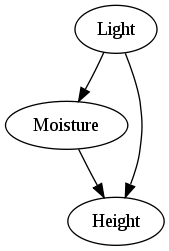
\includegraphics[scale=0.85]{PlantGrowth.png}
    \caption{Bayes Net considered within the plant growth study}
    \label{BNPlant}
  \end{center}
\end{figure}

Both variables $Light$ and $Moisture$ are categorical variables whith the following attributes :  
\begin{itemize}
   \item $Light$ has 2 attributes : $Dim$ which refers to the darkness and $Bright$ which refers to plain light situations,
   \item $Moisture$ has 2 attributes : $Dry$ which refers to dry air situations and $Wet$ which refers to wet air situations.
\end{itemize}
$Height$ is a continuous variable which has to be discretized for the Bayes Net use. \\

The next step is the quantification of the  Bayes Net. According to the data, we propose the following quantification. \\
The variable $Light$ is quantified as follows : 
\begin{itemize}
   \item  $Light="Dim$ with a probability of 0.25,
   \item  $Light=Bright$ with a probability of 0.75.
\end{itemize}

The influence of $Light$ on $Moisture$ is modelized by :
\begin{itemize}
   \item when $Light=Dim$ then  $Moisture=Dry$ with a probability of 0.2 and  $Moisture=Wet$ with a probability of 0.8,
   \item when $Light=Bright$ then  $Moisture=Dry$ with a probability of 0.6 and  $Moisture=Wet$ with a probability of 0.4.
\end{itemize}

The influence of $(Light, Moisture)$ on $Height$ is modelized by :
\begin{itemize}
   \item when $Light=Dim$ and $Moisture=Dry$ then $Height$ follows a $Uniform(min=0, max=20)$ distribution,
   \item when $Light=Dim$ and $Moisture=Wet$ then $Height$ follows a $Triangular(min=15, mod=30, max=50)$ distribution,
   \item when $Light=Bright$ and $Moisture=Dry$ then $Height$ follows a $Triangular(min=0, mod=15, max=30)$ distribution,
   \item when $Light=Bright$ and $Moisture=Wet$ then $Height$ follows a $Normal(\mu=90, \sigma=10)$ distribution.
\end{itemize}


\subsubsection{Some results}

We can study the plant growth variability in different situations like  : 
\begin{itemize}
   \item  I put my plant on my balcony : see Figures \ref{PDFHeight} and \ref{CDFHeight}. In that situation, I set none evidence inside the Bayes Net.
   \item  I put my plant in a  place where it is dark all time (in my cellar?) : see Figures \ref{PDFHeightDim} and \ref{CDFHeightDim}. In that situation, I set one evidence inside the Bayes Net : $Light=Dim$.
   \item  I put my plant in a  place where it is moist all time (in my bathroom?) : see Figures \ref{PDFHeightWet} and \ref{CDFHeightWet}. In that situation, I set one evidence inside the Bayes Net : $Moisture=Wet$.
\end{itemize}




\begin{figure}[H]
  \begin{minipage}{10cm}
    \begin{center}
      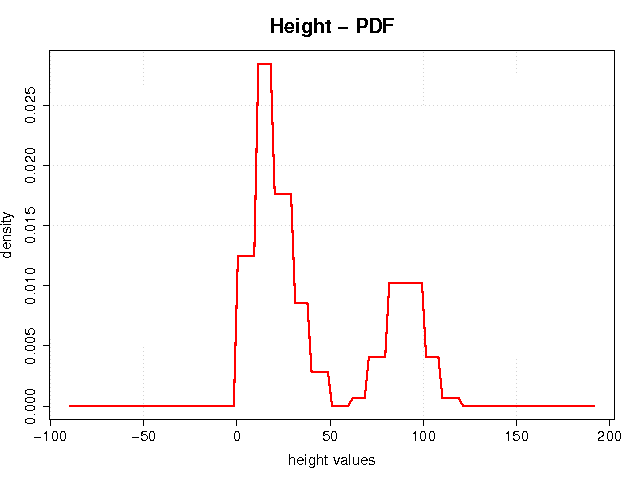
\includegraphics[width=7cm]{Height_PDF.png}
      \caption{Variability of the plant growth on my balcony.}
      \label{PDFHeight}
    \end{center}
  \end{minipage}
  \hfill
  \begin{minipage}{10cm}
    \begin{center}
      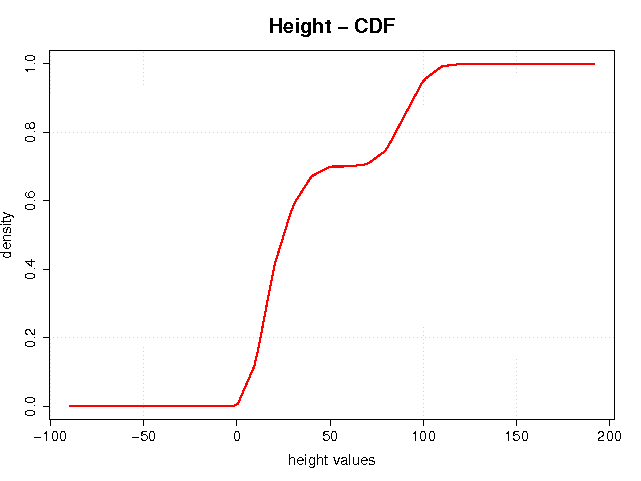
\includegraphics[width=7cm]{Height_CDF.png}
      \caption{Variability of the plant growth on my balcony.}
      \label{CDFHeight}
    \end{center}
  \end{minipage}
\end{figure}



\begin{figure}[H]
  \begin{minipage}{10cm}
    \begin{center}
      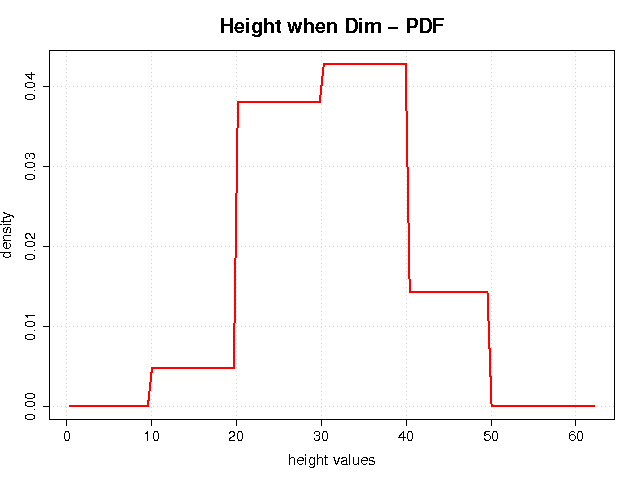
\includegraphics[width=7cm]{Height_PDF_WhenDim.png}
      \caption{Variability of the plant growth in my cellar.}
      \label{PDFHeightDim}
    \end{center}
  \end{minipage}
  \hfill
  \begin{minipage}{10cm}
    \begin{center}
      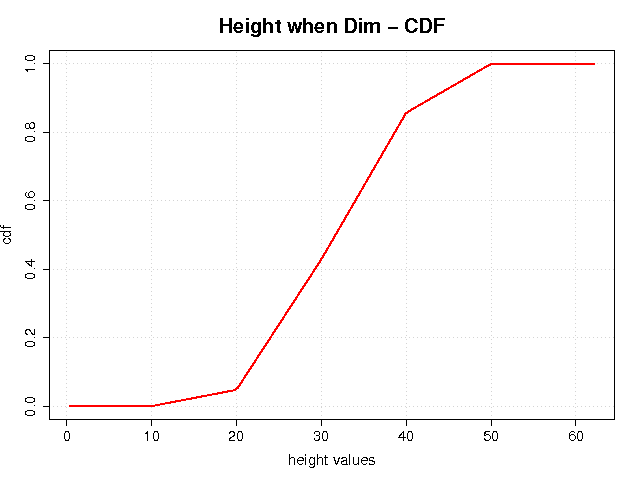
\includegraphics[width=7cm]{Height_CDF_WhenDim.png}
      \caption{Variability of the plant growth in in my cellar.}
      \label{CDFHeightDim}
    \end{center}
  \end{minipage}
\end{figure}


\begin{figure}[H]
  \begin{minipage}{10cm}
    \begin{center}
      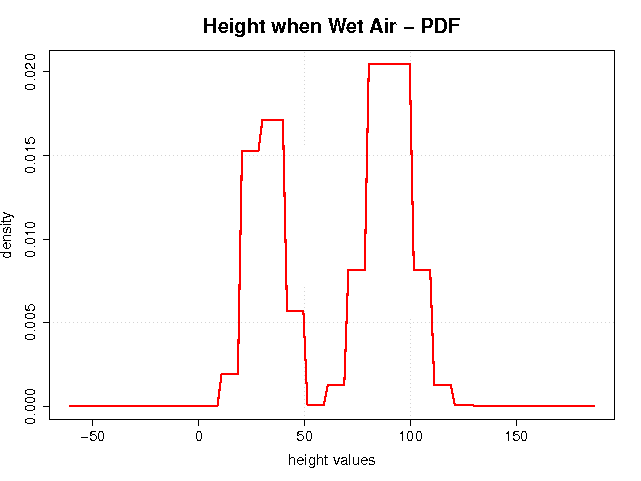
\includegraphics[width=7cm]{Height_PDF_WhenWet.png}
      \caption{Variability of the plant growth in my bathroom.}
      \label{PDFHeightWet}
    \end{center}
  \end{minipage}
  \hfill
  \begin{minipage}{10cm}
    \begin{center}
      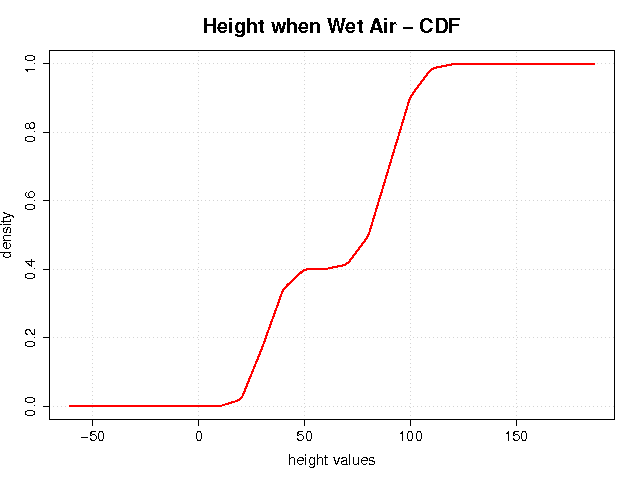
\includegraphics[width=7cm]{Height_CDF_WhenWet.png}
      \caption{Variability of the plant growth in in my bathroom.}
      \label{CDFHeightWet}
    \end{center}
  \end{minipage}
\end{figure}






\subsubsection{Python script}


\begin{lstlisting}
# Load OpenTURNS to manipulate distributions
from openturns import *
# Load pyAgrum to define the Network
from pyAgrum import *
# Load the link between OT and aGrUM
from otagrum import *

# Create an empty BN
netName = "Plant Growth"
myBN = BayesNet(netName)

# Create variables
# LabelizedVar(name, comment, modalities number)
# DiscretizedVar(name, comment)
light = LabelizedVar("Light", "quality of light", 0)
moisture = LabelizedVar("Moisture", "quantity of moisture", 0)
height = DiscretizedVar("Height", "plant growth")

# Create labels and ticks
# light has 2 attributes : Dim and Bright
light.addLabel("Dim")
light.addLabel("Bright")
lightSize = len(light)

# moisture has 2 attributes : Dry and Wet
moisture.addLabel("Dry")
moisture.addLabel("Wet")
moistureSize = len(moisture)


# height has a conditional probability table
# We give here its conditional distributions
# We use some OT distributions
# distribution when Dim and Dry
heightWhenDimAndDry = Uniform(0.0, 20.0)
# distribution when Dim and Wet
heightWhenDimAndWet = Triangular(15.0, 30.0, 50.0)
# distribution when Bright and Dry
heightWhenBrightAndDry = Triangular(0.0, 15.0, 30.0)
# distribution when Bright and Wet
heightWhenBrightAndWet = Normal(90.0, 10.0)

# height is a discretized variable
# We give here its discretized range
data = NumericalPoint(range(0, 180, 10))
# We adapt here its range to its conditional distributions
data = BayesNetAgrum.AdaptGrid(DistributionCollection([
        heightWhenDimAndDry, heightWhenDimAndWet, 
        heightWhenBrightAndDry, heightWhenBrightAndWet
                                                       ]), data)
# We create here the bounds of each local range
#heightSize = data.getSize() - 1
for i in data:
    height.addTick(i)

# Add variables to the net
indexLight    = myBN.add(light)
indexMoisture = myBN.add(moisture)
indexHeight   = myBN.add(height)

# Create arcs
myBN.insertArc(indexLight, indexMoisture)
myBN.insertArc(indexLight, indexHeight)
myBN.insertArc(indexMoisture, indexHeight)

# Create conditional probability tables
# light conditional probability table
myBN.cpt(indexLight)[:]= [0.25, 0.75]

# moisture conditional probability table
# We show the antecedents of moisture with the order in which they were declared
print "moisture Antecedents= ", myBN.cpt(indexMoisture).var_names
myBN.cpt(indexMoisture)[{'Light' : 'Dim'}] = [0.2, 0.8]
myBN.cpt(indexMoisture)[{'Light' : 'Bright'}] = [0.6, 0.4]

# We have to enter some OT distributions 
# whithin aGrUM conditional probability tables
# We show the antecedents of height with the order in which they were declared
print "meight Antecedents= ", myBN.cpt(indexHeight).var_names
# The new class BayesNetAgrum from otagrum is able to marry 
# OT distributions and Agrum conditional probability tables
myBN.cpt(indexHeight)[{'Light': 'Dim', 'Moisture': 'Dry'}]   = 
                BayesNetAgrum.Discretize(heightWhenDimAndDry, data)
myBN.cpt(indexHeight)[{'Light': 'Bright', 'Moisture': 'Dry'}] =
                BayesNetAgrum.Discretize(heightWhenBrightAndDry, data)
myBN.cpt(indexHeight)[{'Light': 'Dim', 'Moisture': 'Wet'}]    = 
                BayesNetAgrum.Discretize(heightWhenDimAndWet, data)
myBN.cpt(indexHeight)[{'Light': 'Bright', 'Moisture': 'Wet'}] = 
                BayesNetAgrum.Discretize(heightWhenBrightAndWet, data)

# Create a BayesNetAgrum object
otbn = BayesNetAgrum(myBN)

# We want to visualize the bayesian network 
# Export to BIF file
otbn.exportToBIFFile(netName+".bif")
# Visualize the graph
otbn.draw(netName)


# Get the distribution of the variable "Height"
heightDistribution = otbn.getMarginal("Height")

# You are whithin Open TURNS : use the distribution the way you want
# Print its caracteristics
print "heightDistribution =", heightDistribution
# Draw its PDf and CDF
heightDistributionPDF = heightDistribution.drawPDF()
heightDistributionPDF.setTitle("Height - PDF")
heightDistributionPDF.setXTitle("height values")
heightDistributionPDF.setYTitle("density")
heightDistributionPDF_draw = heightDistributionPDF.getDrawable(0)
heightDistributionPDF_draw.setLegendName("")
heightDistributionPDF.setDrawable(heightDistributionPDF_draw,0)
heightDistributionPDF.draw("Height_PDF")
heightDistributionCDF = heightDistribution.drawCDF()
heightDistributionCDF.setTitle("Height - CDF")
heightDistributionCDF.setXTitle("height values")
heightDistributionCDF.setYTitle("density")
heightDistributionCDF_draw = heightDistributionCDF.getDrawable(0)
heightDistributionCDF_draw.setLegendName("")
heightDistributionCDF.setDrawable(heightDistributionCDF_draw,0)
heightDistributionCDF.draw("Height_CDF")


# Perform inference

##############################################################
# Example 1 : it is sunny : "Light" == "Bright"

# First, set evidence
otbn.setEvidence("Light", "Bright")

# Get the distribution of the variable "Height"
heightDistribution_Bright = otbn.getMarginal("Height")

# You are whithin Open TURNS : use the distribution the way you want
# Print its caracteristics
print "Height Distribution when Bright =", heightDistribution_Bright
print "Probability (height > 40cm) = ", 1-heightDistribution_Bright.computeCDF(40)
print ""
# Draw its PDF and CDF
heightDistributionPDF_Bright = heightDistribution_Bright.drawPDF()
heightDistributionPDF_Bright.setTitle("Height when Bright - PDF")
heightDistributionPDF_Bright.setXTitle("height values")
heightDistributionPDF_Bright.setYTitle("density")
heightDistributionPDF_Bright_draw = heightDistributionPDF_Bright.getDrawable(0)
heightDistributionPDF_Bright_draw.setLegendName("")
heightDistributionPDF_Bright.setDrawable(heightDistributionPDF_Bright_draw,0)
heightDistributionPDF_Bright.draw("Height_PDF_WhenBright")

heightDistributionCDF_Bright = heightDistribution_Bright.drawCDF()
heightDistributionCDF_Bright.setTitle("Height when Bright - CDF")
heightDistributionCDF_Bright.setXTitle("height values")
heightDistributionCDF_Bright.setYTitle("cdf")
heightDistributionCDF_Bright_draw = heightDistributionCDF_Bright.getDrawable(0)
heightDistributionCDF_Bright_draw.setLegendName("")
heightDistributionCDF_Bright.setDrawable(heightDistributionCDF_Bright_draw,0)
heightDistributionCDF_Bright.draw("Height_CDF_WhenBright")

##############################################################
# Example 2 : the atmosphere is very wet : "Moisture" == "Wet"

# First, erase previous evidences!
otbn.eraseEvidences()
# Set evidence
otbn.setEvidence("Moisture", "Wet")

# Get the distribution of the variable "Light"
lightDistribution_Wet = otbn.getMarginal("Light")
print "Light distribution when Wet Air = "
print "Proba(Dim) = ", lightDistribution_Wet.getParametersCollection()[0][0]
print "Proba(Bright) = ", lightDistribution_Wet.getParametersCollection()[0][1]
print ""

# Get the distribution of the variable "Height"
heightDistribution_Wet = otbn.getMarginal("Height")

# You are whithin Open TURNS : use the distribution the way you want
# Print its caracteristics
print "Height Distribution when Wet Air =", heightDistribution_Wet
print "Probability (height > 40cm) = ", 1-heightDistribution_Wet.computeCDF(40)
print ""
# Draw its PDF and CDF
heightDistributionPDF_Wet = heightDistribution_Wet.drawPDF()
heightDistributionPDF_Wet.setTitle("Height when Wet Air - PDF")
heightDistributionPDF_Wet.setXTitle("height values")
heightDistributionPDF_Wet.setYTitle("density")
heightDistributionPDF_Wet_draw = heightDistributionPDF_Wet.getDrawable(0)
heightDistributionPDF_Wet_draw.setLegendName("")
heightDistributionPDF_Wet.setDrawable(heightDistributionPDF_Wet_draw,0)
heightDistributionPDF_Wet.draw("Height_PDF_WhenWet")
heightDistributionCDF_Wet = heightDistribution_Wet.drawCDF()
heightDistributionCDF_Wet.setTitle("Height when Wet Air - CDF")
heightDistributionCDF_Wet.setXTitle("height values")
heightDistributionCDF_Wet.setYTitle("density")
heightDistributionCDF_Wet_draw = heightDistributionCDF_Wet.getDrawable(0)
heightDistributionCDF_Wet_draw.setLegendName("")
heightDistributionCDF_Wet.setDrawable(heightDistributionCDF_Wet_draw,0)
heightDistributionCDF_Wet.draw("Height_CDF_WhenWet")


##############################################################
# Example 3 : there is no light : "Light" == "Dim"

# First, add one more  evidence
otbn.setEvidence("Light", "Dim")

# Get the distribution of the variable "Height"
heightDistribution_Dim = otbn.getMarginal("Height")

# You are whithin Open TURNS : use the distribution the way you want
# Print its caracteristics
print "Height Distribution when Dim =", heightDistribution_Dim
print "Probability (height > 40cm) = ", 1-heightDistribution_Dim.computeCDF(40)
print ""
# Draw its PDf and CDF
heightDistributionPDF_Dim = heightDistribution_Dim.drawPDF()
heightDistributionPDF_Dim.setTitle("Height when Dim - PDF")
heightDistributionPDF_Dim.setXTitle("height values")
heightDistributionPDF_Dim.setYTitle("density")
heightDistributionPDF_Dim_draw = heightDistributionPDF_Dim.getDrawable(0)
heightDistributionPDF_Dim_draw.setLegendName("")
heightDistributionPDF_Dim.setDrawable(heightDistributionPDF_Dim_draw,0)
heightDistributionPDF_Dim.draw("Height_PDF_WhenDim")

heightDistributionCDF_Dim = heightDistribution_Dim.drawCDF()
heightDistributionCDF_Dim.setTitle("Height when Dim - CDF")
heightDistributionCDF_Dim.setXTitle("height values")
heightDistributionCDF_Dim.setYTitle("cdf")
heightDistributionCDF_Dim_draw = heightDistributionCDF_Dim.getDrawable(0)
heightDistributionCDF_Dim_draw.setLegendName("")
heightDistributionCDF_Dim.setDrawable(heightDistributionCDF_Dim_draw,0)
heightDistributionCDF_Dim.draw("Height_CDF_WhenDim")
\end{lstlisting}









%%%%%%%%%%%%%%%%%%%%%%%%%%%%%%%%%%%%%%%%%%%%%
\newpage \subsection{Your study}

It's up to you to propose one new very interesting example! ...

\printindex
\end{document}
